
\documentclass[12pt]{report}
\usepackage{graphicx}
\usepackage{amsmath}
\begin{document}

\tableofcontents

%\chapter{IGS-based diversity analysis}

\chapter{concept and simulation}

\section{Introduction}

In almost all  metagenomics projects, diversity analysis plays an important
role to supply information about the richness of species, the species abundance
distribution in a sample or the similarity and difference between different 
samples, all of which are crucial to draw insightful and reliable conclusion. 
Traditionally especially for amplicon metagenomics data set, OTUs(Operational 
Taxonomic Units) based on 16S rRNA genes are used as the basic units for 
diversity analysis. OTUs can be good replacement of the concept of "species" in 
metagenomics. Basically contigs are assembled from reads and are "binned" into
OTUs using composition-based or similarity-based approaches. Then the diversity
can be estimated by using the abundance information of the OTUs.

% from proposal, need to be rewritten to be more precise.
Recently there are many more projects generating whole genome shotgun metagenomics data sets. However they are 
mainly used for assembly and annotation purpose. Less attention was paid to diversity measurement
using these whole genome metagenomics data sets. One possible reason is that the whole genome metagenomics
data sets are often with low depth given the high diversity of metagenomics samples compared to 16S rRNA
ampicon metagenomics data set. Assembly and annotation are always challenging with the low depth and lack of 
reference sequences. It is also true for diversity measurement. On the other hand, although with low depth, some whole genome metagenomics 
data sets are with large size because of the high diversity. For instance, there may be 4 petabase
pairs of DNA in a gram of soil{Zarraonaindia:2013aa}. Many of those methods for sequence binning or diversity 
estimation do not scale well and will not work for large metagenomics data sets. For instance,
many composition-based binning approach involves k-mer/signature frequency distribution calculation, which is 
rather computationally expensive. Even basic sequence alignment will be impossible for large metagenomics data set.
Many of those statistical software packages to estimate diversity using various estimators are not prepared 
for the large scale of whole genome metagenomics data. 

With the development of next generation sequencing technology, the cost of sequencing is dropping rapidly. 
Whole genome metagenomics sequencing is more popular and large amount of metagenomics data is 
being generated with increasing speed, which can not be even met by the increase of computational capacity.
Novel methods that can scale well are extremely needed to deal with the increasingly large metagenomics data
set. 


%diversity analysis, is the central topic of in microbial ecology.
%
%
%1. traditionally, OTU 
%
%2. assembly, annotation, 
%megan, 
%
%binning
%
%3. co abundance methods.
%
%4. alpha , genome size estimation.
%
%5. igs, better , advantage
%
%alpha, beta 
%
%
%
%assembly, contig binning
%
%no assembly, no reference sequence
%
%
%kmer couting, 
%
%paper:
%
%alpha, co abundance, 
%beta, co abundance across samples
%
%
%
%
%khmer counting,
%
%streaming, diginorm, 
%


Here we propose a novel concept - IGS (informative genomic 
segment) and use IGS as a replacement of OTUs to be the cornerstone for 
diversity analysis of whole shotgun metagenomics data sets. IGSs represent the 
unique information in a metagenomics data set and the abundance of IGSs in 
different samples can be retrieved by the reads coverage through an efficient 
k-mer counting method. This samples-by-IGS abundance data matrix is a promising
replacement of samples-by-OTU data matrix used in 16S rRNA based analysis and 
all existing statistical methods can be borrowed to work on the samples-by-IGS 
data matrix to investigate the diversity. We applied the IGS-based method to 
several simulated data sets and a real data set - Global Ocean Sampling 
Expedition (GOS) to do beta-diversity analysis and the samples were clustered 
more accurately than existing alignment-based method. We also tried this novel 
method to Great Prairie Soil Metagenome Grand Challenge data sets. Furthermore 
we will show some preliminary results using the IGS-based method for 
alpha-diversity analysis. Since this method is totally binning-free, 
assembly-free, annotation-free, reference-free, it is specifically promising 
to deal with the highly diverse samples, while we are facing large amount of 
“dark matters” in it, like soil.




\section{The concept of IGS(informational genomic segment)}

In classic ecology dealing with macroorganisms, diversity measurement is based 
on the concept of species. For 16S rRNA amplicon metagenomics data set, it is 
based on the concept of OTUs. While the concept of OTUs can be used to analyze
large shotgun metagenomics data set, normally assembly, binning and annotation
are required before doing diversity analysis. However these are difficult
tasks, lacking of necessary reference genome or being computationally
expensive. So we are interested in finding an approach to bypass the difficult
tasks like assembly, binning, annotation and use raw reads to make diversity
analysis to large metagenomic data possibile. In the beginning we proposed that
 the concept of k-mers(a DNA segment with the leng of k) can be used to measure
 diversity. K-mers can be considered as the atom of information in DNA 
sequences. One of the composition-based approaches to binning is to use the 
k-mer as the signatures. Suppose the sizes of microbial genomes are similar and
 the difference between genomic content of microbial genomes is similar, the 
number of distinct k-mers in the sequence data set correlates to the number of 
species in a sample. However, because of sequencing error, which is unavoidable
 due to the limit of sequencing technology, this k-mer based analysis doe not 
work well. One sequencing error on a read will generate at most k erroneous 
k-mers. In metagenomics data set, especially with high coverage, most of the 
distinct observed k-mers are from sequencing errors.
%add citation about k-mer based diversity analysis ,entropy...
% add some results /figures

Next we looked at the upper level - reads. A novel method termed as digital 
normalization was developed to remove abundant reads before assembly. However 
it also supplies a novel way to distil information from reads by reducing the
 bad effect of sequencing errors so that we can use those informative reads to 
measure the microbial diversity. We term those informative reads as 
IGS(informative genomic segment), which can be considered as a segment of DNA 
on a microbial genome. Those IGSs should be different enough to represent the 
abstract information a genome contains. Suppose microbial genomes contain 
similar number of those IGSs, as they contain similar number of distinct 
k-mers, the number of IGSs will correlates with the species richness in a 
sample, and the abundance distribution of IGSs will be related to species 
evenness in a sample. Furthermore, we can get the abundance of the IGSs across
different samples. Many classic diversity estimation methods based on OTUs 
 described in sections above can be applied to estimate the diversity of IGSs 
and the diversity of actual species subsequently.

The concept of IGS can be the foundation of a novel statistical framwork to
evaluate microbial diversity using whole genome shotgun metagenomic data, 
especially while facing large amount of "dark matters", unknown species. It is
almost impossible to do annotation to those "dark matters", since we do not
have much information about them. 
% need expanding
For alpha diversity, we can generate a list of IGSs and the respective 
abundance in a sample. Then existing estimators like Chao's can be used to 
estimate the total number of IGSs in the sample. Rarefaction curve based on 
number of IGSs can also be generated. 

% need expand the discussion from IGS in one sample to IGS in different samples.
For beta diversity, we can generate a samples-by-IGS data matrix from the
abundance of IGSs across samples, as a replacement of samples-by-OTU data 
matrix in OTU-based analysis and samples-by-species data matrix in traditional 
ecology. From that samples-by-IGS data matrix, we can use existing methods to 
calculate similarity/disimilarity/distance between samples and do further 
analysis like clustering and ordination. 

% further application
% With the samples-by-IGS data matrix, it is also possible to calculate similarity between IGSs and do ordination, which is a potential approach to classify IGS( reads).

%Using simulated and real genomic data sets, with the help of khmer to get median k- mer abundance, we find that median k-mer abundance correlates well with mapping-based coverage.

%Side note: We can also see that the coverage by median k-mer count is generally lower than the read coverage by mapping. So estimation of sequencing coverage by median k-mer count is underestimated. This can cause some problems in later analysis, which will be discussed later.


\subsection{IGS(informative genomic segment) can represent the novel 
information of a genome}

Median k-mer abundance can represent sequencing depth of a read(cite diginorm).
 For a sequencing reads data set with multiple species, the sequencing depth of
 a read is related to the abundance of species where the read originates. 

% figure 1a should be marked 
The Figure \ref{fig:reads_to_IGS}a  shows the abundance distribution of reads 
from 4 simulated sequencing data sets with different sequencing depth - 3 
sequencing data sets generated with different sequencing coverage(1x, 10x, 40x)
 from 3 simulated random genomes respectively and 1 combined data set with all 
the previously mentioned data sets. No error is introduced in these simulated 
data sets. Obviously the reads from the three data sets can be separated by 
estimated sequencing depth. The combined data set can be considered as a 
sequencing data set with three species with different abundance.

Each point on the curve shows that there are Y reads with a sequencing depth of
 X. In other word, for each of those Y reads, there are X-1 other reads that 
cover the same DNA segment in a genome that single read originates. So we can 
estimate that there are Y/X distinct DNA segments with reads coverage as X. 
We term these distinct DNA segments in species genome as 
IGS(informative genomic segment). We can transform the figure in upper 
position to show the number of IGSs and their respective reads coverage, as 
shown in figure in lower position. We sum up the numbers of IGSs with 
different reads coverage for each data set and get the result as shown in 
below. The sum numbers of IGSs here essentially are the areas below each curve 
in the figure.

Even though the datasets have different sequencing depth like 10X and 40X, 
they have similar numbers of IGSs. Dataset with 1X sequencing depth has fewer 
IGSs because the depth is not enough to cover all the content of the 
genome(63.2\%). The IGSs can be seen as the
genomic segment on a genome with the length of reads.(Figure \ref{fig:IGS}  
Assume the species 
genome is totally random, which is the case in the simulated data set, the 
number of IGSs(N) in a species genome is related to the size of genome(G), 
read length(L) and k size(k), which can be denoted as

\[N =\frac{G}{L}  \]
which is the number of reads that can have a 1X coverage of the genome.
For the simulated genome with size of 1M bps, read length as 80bps, expected 
number of IGSs is 

1000000/(80 - 22 + 1) = 16949, 

which is pretty close to observed value. See Table \ref{table:IGSs}
((((((( This needs rewrite, the table will be replaced)))))))))))

\begin{figure}[!ht]
\centerline{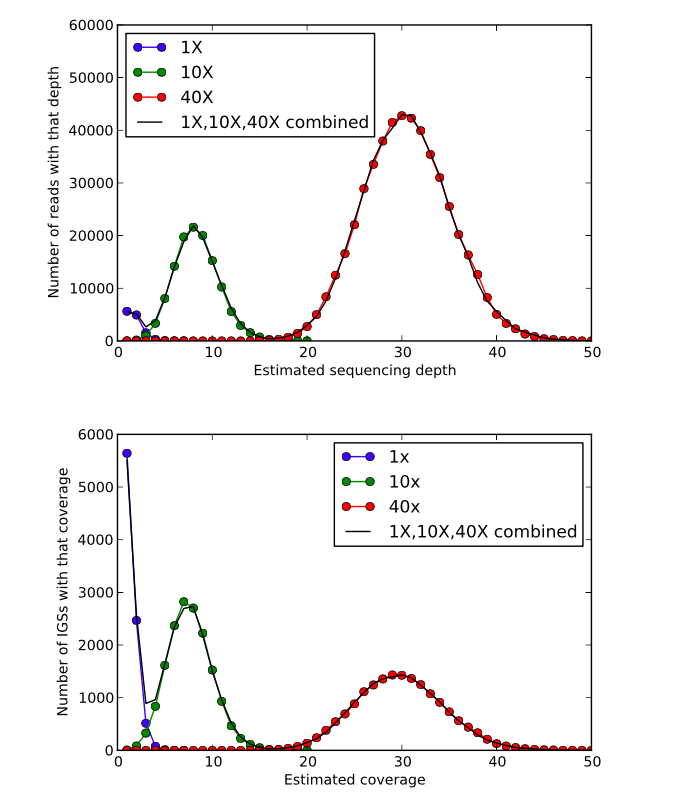
\includegraphics[width=4in]{./figures/from_reads_to_IGS.png}}
%\caption{\bf cluster of GOS samples using IGS method}
\caption{\bf from reads to IGS}
\label{fig:reads_to_IGS}
\end{figure}

\begin{table}[!ht]
\caption{
\bf{Total number of IGSs in different simulated reads data sets.}
}
\begin{tabular}{ |c | c |c| c|c| }
Data set & total number of IGSs \\
\hline \\
1X depth                   & 8714  \\
10X depth                  & 16321  \\
40X depth                  & 16794 \\
1X,10X,40X combined        & 41742 \\
\end{tabular}
\begin{flushleft}
\end{flushleft}
\label{table:IGSs}
\end{table}


\begin{figure}[!ht]
\centerline{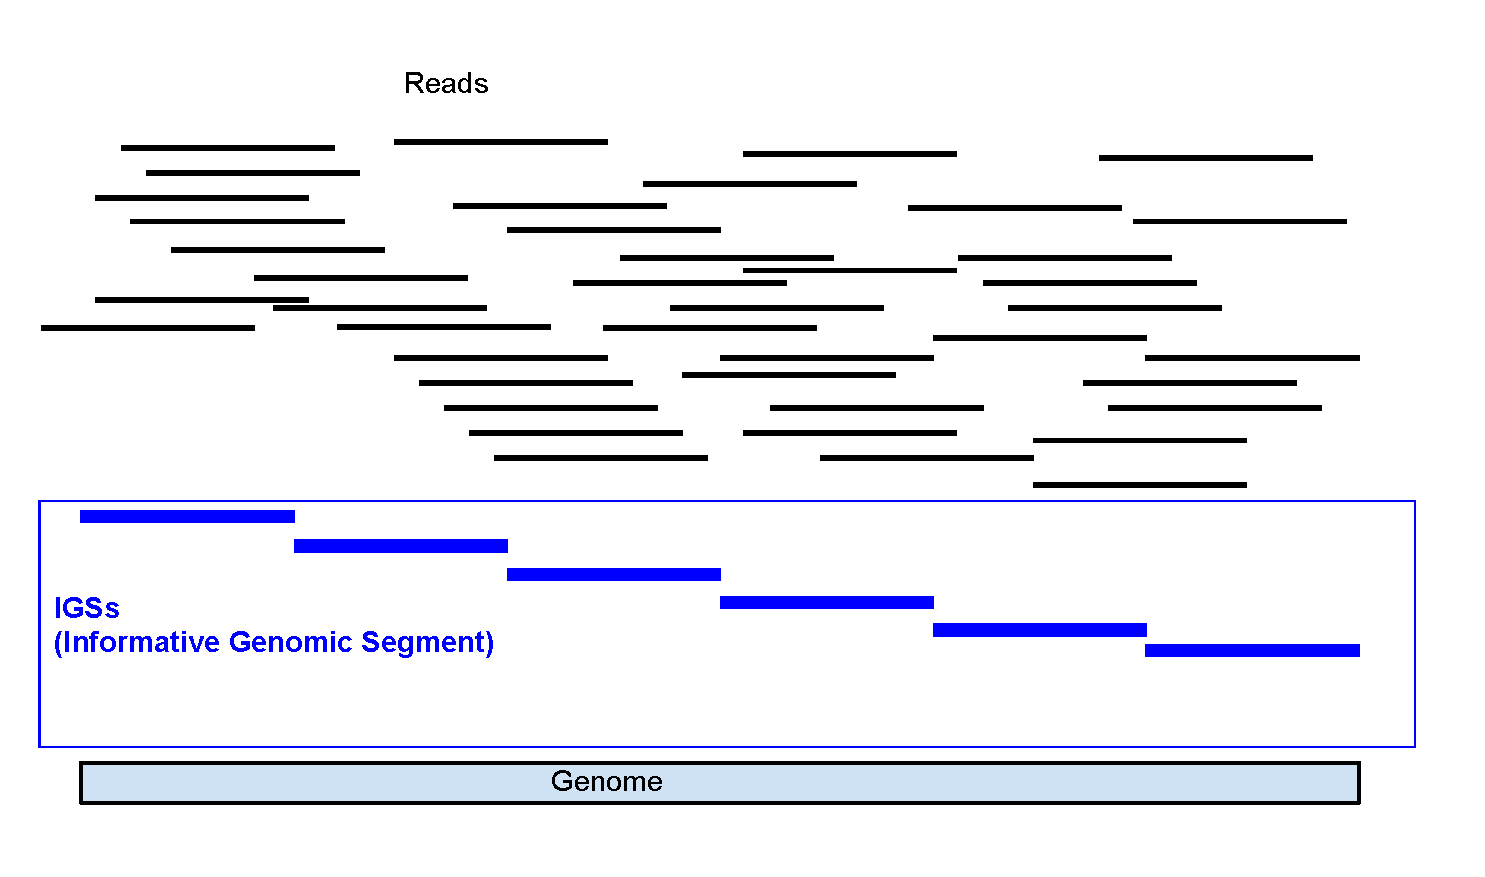
\includegraphics[width=4in]{./figures/IGSs_figure.pdf}}
\caption{\bf the concept of IGS}
\label{fig:IGS}
\end{figure}





\subsection{IGS can be used to do alpha diversity analysis}

Basically the abundance distribution of IGSs with different coverage in a sample data set is acquired using the method shown above, like:
\\
3 23\\
4 24\\
5 25\\
6 25\\
...\\
\\
Here 23 IGSs with coverage as 3, this number is calculated from dividing the total number of reads with coverage as 3, which is 69, by the coverage 3: 69/3. Similarly there are 96/4 = 24 IGSs with coverage as 4.

If we draw an analogy between IGSs and OTUs, this is like there are 23 different OTUs with 3 reads mapped to, and 24 different OTUs with 4 reads mapped to. 

Then list all the different IGSs and the corresponding count,and we can get a long list with each IGS and the corresponding coverage.The coverage of an IGS can be considered as the abundance of such IGS in a sample. The list looks like:
\\
IGS\_ID abundance\\
1     3\\
2     3\\
3     3\\
 ...\\
23    3\\
24    4\\
25    4\\
...\\
47    4\\
48    5\\
 ...\\
 ...\\
  
This list is the counterpart of an OTU table in OTU based diversity analysis.

With such table at hand, numerous existing statistical methods and software packages can be used to investigate the alpha diversity.  



\subsection{IGS can be used to do beta diversity analysis}

As in alpha diversity analysis, OTU table is also a cornerstone for beta diversity analysis. As long as we get a reliable OTU table, there are existing pipelines to do the beta diversity analysis. 

A typical OTU table across different samples is like this, which is also called samples-by-OTU data matrix.
\\
OTU\_ID Sample1\_ID Sample2\_ID Sample3\_ID\\
OTU1   3          4          2\\
OTU2   2          5          0\\
OTU3   3          1          4\\
\\
    
Like a OTU table, we hope to have the IGS table for the IGSs:
\\
    IGS\_ID SampleA SampleB SampleC SampleD\\
    IGS1   5       1       2       1\\
    IGS2   5       1       2       1\\
\\
    
    So now the problem is how we can generate a sample-by-IGS data matrix as the counterpart of samples-by-OTU data matrix so many of  the existing tools/methods used for OTU-based diversity can be borrowed for this kind of IGS-based analysis, just as what is shown above for alpha diversity analysis.

Firstly, as how we get the coverage of a read from a sample dataset in this sample dataset, we can get the coverage of a read from a sample A dataset in another sample B dataset. We can still use the median k-mer count to represent the coverage. The basic idea is the same. 

Because a read must derive from a segment in the genome of some species in a sample, if a read R from sample A with a coverage C\_A in sample A has a coverage as C\_B in sample B, that means that segment of genome in sample A from which read R derive also exists in sample B. That genomic segment has a coverage as C\_A in sample A and has a coverage as C\_B in sample B. Roughly there should be about C\_A reads (read R should be one of them) in sampleA covering that genomic segment and C\_B reads in sampleB covering that genomic segment. Meanwhile, the C\_A reads in sampleA should all have a coverage as C\_B in sampleB, just like read R as one of them. Similarly, the C\_B reads in sampleB should all have a coverage as C\_A in sampleA.

Ok, now let's make an example. 

Suppose there are 6 reads in sample A, all have a coverage as 3 in sampleA, and have a coverage as 2 in sampleB.

According to the discussion about IGS in previous section, the 6 reads cover 2 IGSs with a coverage as 3 for each IGSs. There should be 4 reads in sampleB covering the exact same 2 IGSs, with a coverage as 2 in sampleB.

So now we have 2 distinct IGSs with redundancy as 3 and 2 in the two samples respectively. 

**Note:** small number is used in the analysis above as example, but it should be emphasized that the analysis is based on large number statistically.


Let's expand this example from 2 samples to 4 samples(A,B,C,D), as shown in figure above.

Let's say we find 10 reads in sampleA, with coverage as 5-1-2-1 in samples A-B-C-D respectively. (We call "5-1-2-1" "coverage  spectrum" across samples.) So there should be **about** 2 reads in sampleB, 4 reads in sampleC, 2 reads in sampleD, all of which have a "coverage spectrum" as "5-1-2-1". Basically these 18 reads altogether cover 2 distinct IGSs, which apparently exist in all the 4 samples. The 2 distinct IGSs has a redundancy as 5,1,2,1 in the 4 samples respectively.

If we draw an analogy between IGSs and OTUs, this is like there are 2 OTUs, both with 5,1,2,1 reads mapped to in sample A,B,C,D respectively.

Like a OTU table, here we can have the IGS table for the two IGSs:
\\
    IGS\_ID SampleA SampleB SampleC SampleD\\
    IGS1   5       1       2       1\\
    IGS2   5       1       2       1\\
\\
    
 % should all include alpha and beta diversity results
\section{Evaluating IGS method using simulated data sets}
\subsection{An experiment using a simple simulated data sets}

For this experiment, firstly we create 6 synthetic samples (Sample 1-6) based on 9 synthetic 10K genomes (genome A-I), with different composition of species and diversity. 

The  species composition for each synthetic sample is as below:

sample1: AAAB

sample2: AABC

sample3: ABCD

sample4: ABCE

sample5: AFGH

sample6: IFGH

For sample1, there are two species - A and B, with abundance distribution as 3:1.

The sequencing depth of all the synthetic data sets is 10X. So the species abundance in each sample is as below:

sample1: genomeA - 30, genomeB - 10

sample2: genomeA - 20, genomeB - 10, genomeC - 10

sample3: genomeA - 10, genomeB - 10, genomeC - 10, genomeD - 10

sample4: genomeA - 10, genomeB - 10, genomeC - 10, genomeE - 10

sample5: genomeA - 10, genomeF - 10, genomeG - 10, genomeH - 10

sample6: genomeI - 10, genomeF - 10, genomeG - 10, genomeH - 10


An a simple experiment, there is no sequencing errors introduced in the synthetic reads data sets.

Figure \ref{fig:simple_pcoa} and Figure \ref{fig:simple_cluster} show that IGS method can yield the information 
about the difference of samples correctly. Sample 5 and sample 6 and very close to each other on the figure, which 
is true if we check the species composition of the two samples shown above.

Figure \ref{fig:simple_alpha} shows the  method can yield the richness information correctly. From the figure, samples with 
4 different species have the richness almost twice as large as the sample with 2 different species. 

From these results, we show the IGS method can work well to a simplest scenario, with high sequencing depth (10X) and no sequencing error. Next we will check the influence to the analysis accuracy of variable sequencing depth and sequencing error and introduce new ways to preprocess the data to decrease the influence of sequencing error. 


\begin{figure}[!ht]
 \centerline{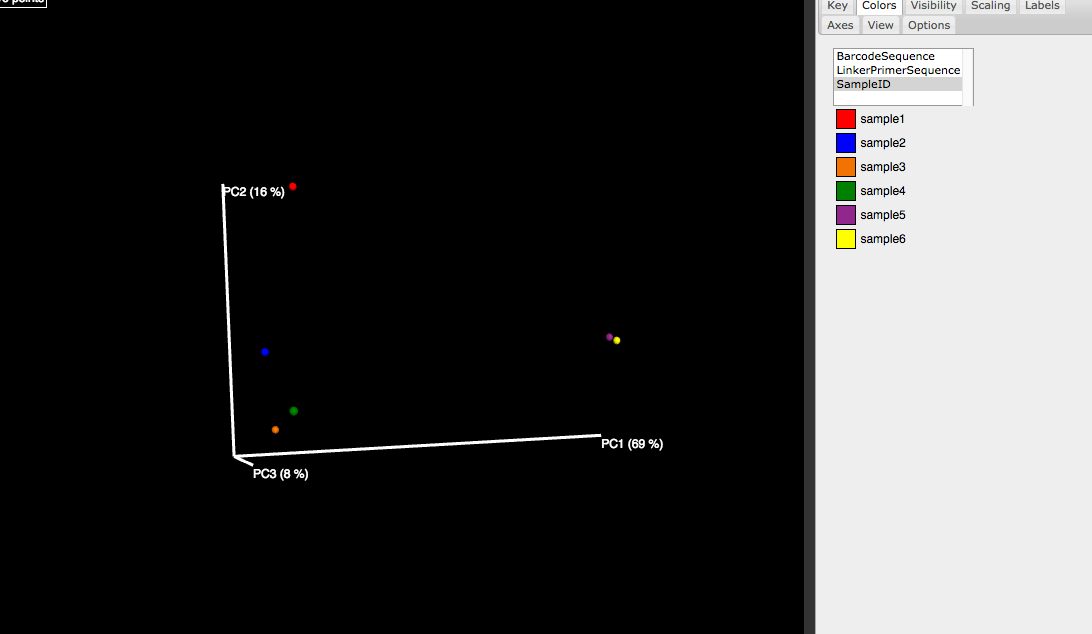
\includegraphics[width=4in]{./figures/simple_PCA_3d.png}}
\caption{\bf Ordination of the 6 synthetic samples using IGS method}
\label{fig:simple_pcoa}
\end{figure}


\begin{figure}[!ht]
 \centerline{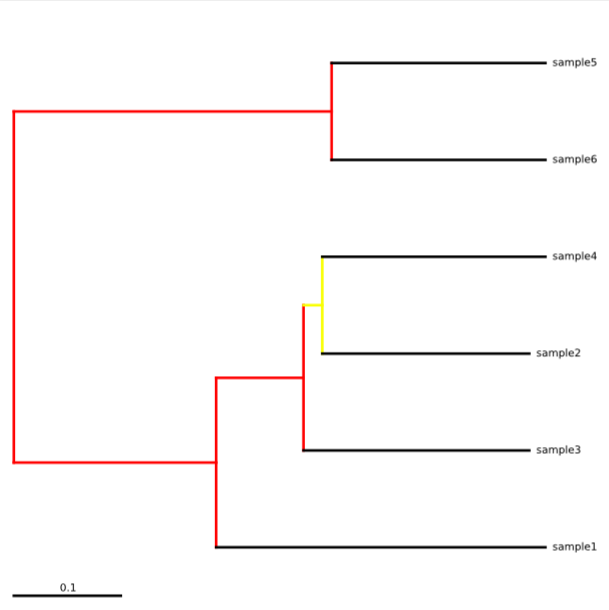
\includegraphics[width=4in]{./figures/simple_tree.png}}
\caption{\bf Clustering of the 6 synthetic samples using IGS method}
\label{fig:simple_cluster}
\end{figure}


\begin{figure}[!ht]
 \centerline{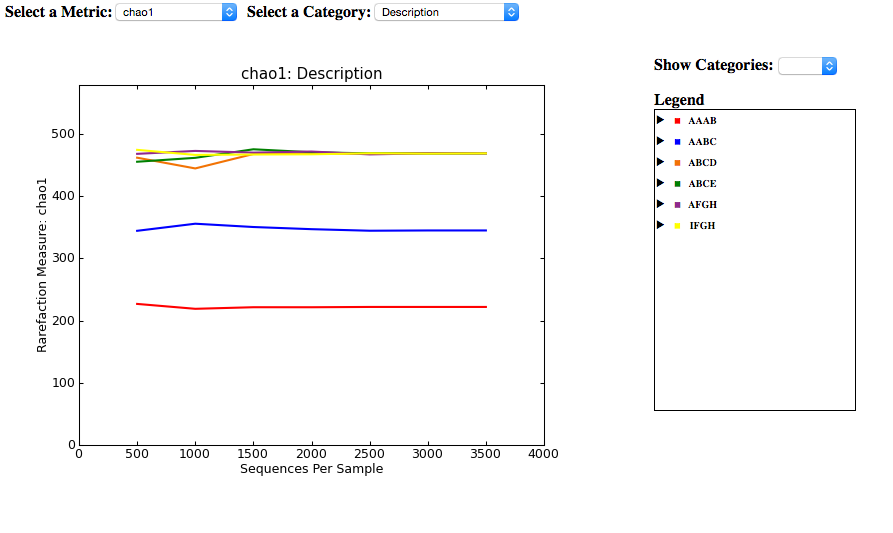
\includegraphics[width=4in]{./figures/simple_chao_alpha.png}}
\caption{\bf Richness estimation of the 6 synthetic samples using IGS method}
\label{fig:simple_alpha}
\end{figure}


\subsection{Improving the accuracy of this method in real world analysis}


Previously we have shown the IGS method generally works to a simple simulated
 data sets, with high sequencing depth and no sequencing error. In real world,
in many situations we have to deal with the metagenomic data sets with 
relatively low sequencing depth, like soil or sea water samples. 
Also it is a fact that all sequencing technology will generate some errors. As 
discussed in the background 
section, one of the reasons we develop the IGS method is that based on the 
abundance counting of reads rather than k-mers, it is expected that the IGS 
method is less prone to sequencing error. However the effect of those factors 
jeopardizing the accuracy is still observable. 

In this section, we will analyze the effect of these factors to the accuracy of
 the IGS method and investigate the ways to reduce the effect to increase the 
accuracy of analysis.


As in last section, six synthetic samples were generated with the same species 
composition . For each sample, sequencing reads data sets with different
sequencing depth(0.1X, 1X, and 10X) and different sequencing error rate (0.5\%,
 1.0\%, 1.5\%, and 0\% - no error at all) are simulated.

To show the effect of sequencing error to accuracy of the 
analysis, we compared the richness estimation using reads with different 
sequencing error rate, as shown in Figure \ref{fig:IGS_richness_no_adjustment}. 
For data set without error (error rate = 0), the esimated size of metagenome
matches real size perfectly. With increasing error rate, the size of metagenome
is over estimated more and more seriously. This is due to several factors,which
will be discussed below. 
\begin{figure}[!ht]
 \centerline{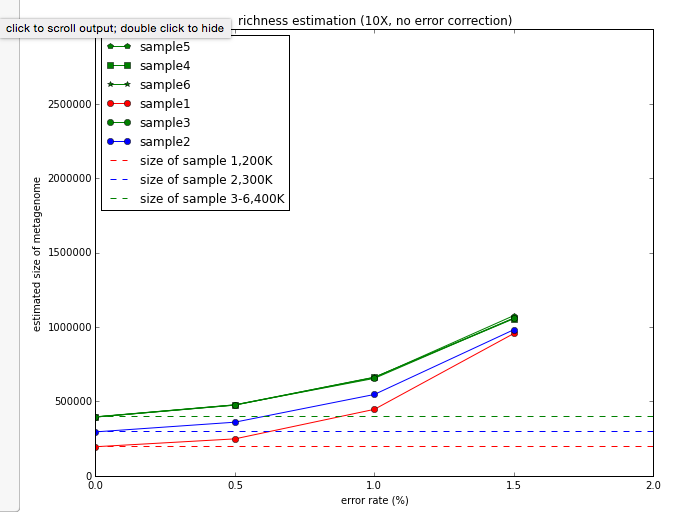
\includegraphics[width=4in]{./figures/IGS_richness_no_adjustment.png}}
\caption{\bf Richness estimation using IGS method without adjustment}
\label{fig:IGS_richness_no_adjustment}
\end{figure}

\subsubsection{the effect of sequencing error to the accuracy of analysis}
The first factor to take into account is sequencing error. One sequencing error
will generate k erroneous k-mers. This is the reason why it is difficult to use
k-mer counting only to do diversity analysis, as a large proportion of k-mers
in a reads data set are erroneous, especially for low coverage reads data. As
discussed in the section about digital normalization, using median k-mer count
to retrieve the coverage of a read is less prone to sequencing error, because
sequencing error will decrease the count of some reads to 1 incorrectly, but
this does not always affect the median k-mer count. 

Take the experiment we did
previously as an example, for read length as 100bp and k as 19, one sequencing
error will affect the count of 19 k-mers at the most, two sequencing errors
will affect the count of at most 38 k-mers. The count of these k-mers will be
retrieved as 1 incorrectly, suppose it is highly impossible that an erroneous
k-mer is the same as another real k-mer in the data set accidently, as long as
the k is large enough compared to the size of data set. So out of the 82 k-mers
in the 100bp read, at most 38 k-mers will have count as 1 incorrectly, but this
will not affect the median k-mer count, which is the count of the 41th k-mer if
ranked by count. However, if there are three or more errors in the read, the 
situation is more complicated. For 3 errors in a read, 3 to 57 k-mers
will be affected by the errors to have an incorrect count as 1. The 
distribution of the probability about the number of affected k-mers can be
acquired by a model similar to Lander-Waterman model used in genome sequencing
 theory. Here we got the distribution using simulation, as shown in Figure
\ref{fig:IGS_affected_k_kmers}. From this probability distribution, we can get
the probability that 3 errors will affect more than 40 k-mers is 0.43. In this
case, 3 errors will affect the median k-mer count of a read. We can also get 
such probability for 4 errors or more. Combining to the probability that a
certain number of errors occur in a read with a specific sequencing error rate,
which is easy to derive from binomial distribution, we can get the probability
that the coverage of a read is incorrectly assessed as 1. Still for the example
here, this probability is the probability that 3 erorrs occur in a read
multiplied by the probability that 3 errors will affect median k-mer count,
plus the probability that 4 erorrs occur in a read multiplied by the 
probability that 4 errors will affect median k-mer count,and so on.

Generally, let $P\_error(n,e,L)$ is the probability that $n$ errors occur in a 
read with length as $L$, with error rate as $e$ and $P\_effect(n,k,L)$ is the 
probability that $n$ 
errors in a read with length of $L$ affect median k-mer count. The probability 
that the coverage of a read is incorrectly assessed as 1 is 
\[\sum_{n=3}^{\infty} P\_error(n,e,L) \times P\_effect(n,k,L)  \],
and by binomial distribution,

\[P\_error(n,e,L) = f(n;L,e) = Pr(X=n) = {L \choose n}e^n(1-e)^{L-n} \] 

Practically, when $n>5$ and $e<0.015$, $P\_error(n,e,L)$ is very small, we only consider
number of errors in a read as 3, 4 and 5.

\begin{figure}[!ht]
 \centerline{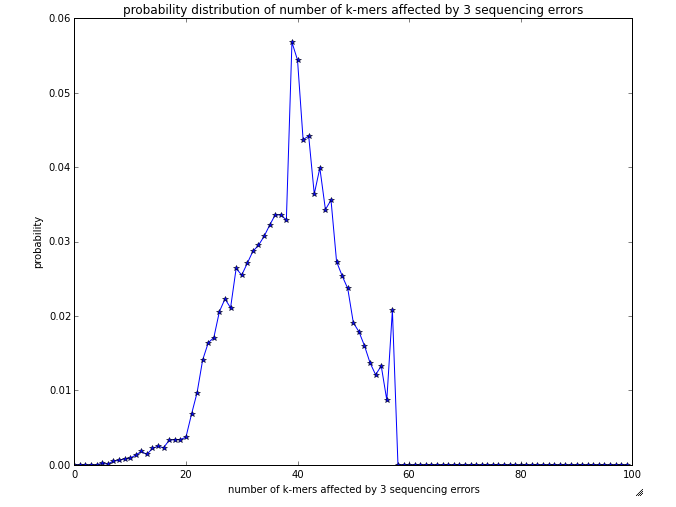
\includegraphics[width=4in]{./figures/IGS_affected_k_kmers.png}}
\caption{\bf Richness estimation using IGS method without adjustment }
\label{fig:IGS_affected_k_kmers}
\end{figure}

From the discussion above, the sequencing errors reduce the coverage of some
reads incorrectly to 1 and the probability this occurs to a read can be
estimated. So to reduce the effect of sequencing error on this aspect, we can
calculate the expected number of reads that are affected and remove those reads
from the set of reads with coverage as 1 before generating list of IGS from the
reads abundance distribution.

Also, we want to make sure 2 errors in a read will not affect median k-mer 
count, since it is more common to have 2 errors in a read practically. 
In this case, 
\[2 \times k < \lfloor \frac{L-k+1}{2}\rfloor \],
we can get $k<L/5$,basically. For $L$ as 100, $k$ will be 19, which is what we 
choose in the testing. However, the $k$ should not be too small, or the k-mers 
can not handle the information of a large data set.

Taking the sequencing error into account, we used the methods introduced above
to adjust the estimation of metagenome size of the 6 synthetic samples. The
estimation after adjustment is closer to real number, as shown in Figure
\ref{fig:IGS_richness_error_adjustment}..


\begin{figure}[!ht]
 \centerline{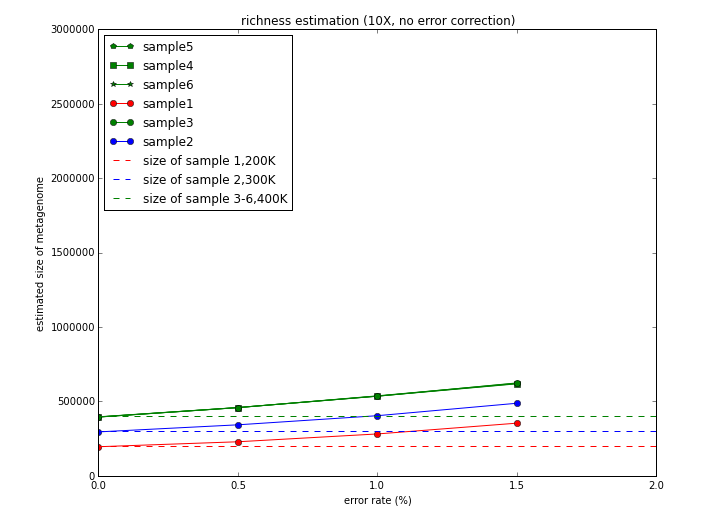
\includegraphics[width=4in]{./figures/IGS_richness_error_adjustment.png}}
\caption{\bf Richness estimation using IGS method adjusted by sequencing error rate}
\label{fig:IGS_richness_error_adjustment}
\end{figure}

\subsubsection{the effect of collision in bloom filter to analysis accuracy}
As discussed in the chapter about k-mer counting, the collision in bloom filter
which we use for efficient k-mer counting will result in counting error. If the
false positive rate for a specific bloom filter we use for k-mer counting is
0.1, 10\% of the k-mers will have incorrect counts. When we use median k-mer
count to get read coverage, such incorrect count has the effect on two aspects.
On one hand, some k-mers in a read will have incorrect higher count. But if the
 false
positive rate is low, this will not affect median k-mer count. This shows the
method of using median k-mer count to get read coverage is not only less prone
to sequencing error, but also less prone to the inaccuracy characteristics of
underlying data structure. One the other hand, this inaccurate count also
affects the counts of those erroneous k-mers generated by sequencing error. For
example, 3 errors in a read affect the count of 43 k-mers, the counts for these
43 k-mers are supposed to be 1. But because of the collision in bloom filter
and the resulting incorrect k-mer counting, if the false positive rate is 0.1,
about 4 out of the 43 k-mers will have inflated count, mostly as 2. So the
combined effect of sequencing error and collision in bloom filter is that some
reads will have incorrect coverage as 1 and some reads will have incorrect as
2. We can get the percentage of total reads that will have such incorrect
coverage, using statistical model similar to that discussed in last section.
Using same example, 3 errors occur in a read, if the 3 errors affect 41-45
k-mers(with a chance of 0.20), the median k-mer count will be 2, due to the 
collison in bloom filter, while if he 3 errors affect more than 45 k-mers(with 
a chance of 0.24), the median k-mer count will be 1, purely due to sequencing 
errors. 

We did the same experiment but also adjusted the estimation according to the 
false positive rate of bloom filter and got better estimation, as shown in
Figure \ref{fig:IGS_richness_adjustment}.

With adjustment to estimation taking sequencing error and collision in bloom
filter into account, as shown in Figure \ref{fig:IGS_richness_adjustment}, the 
estimated genome size is closer to real number. With error rate as 1\%,
false positiver rate as 0.1, with 10X coverage data, the estimated genome size
is about 20-25\% more than real number. However the estimation is still 
increasing with higher
error rate. This means there are still other factors influencing this
accuracy of the estimation but we failed to take into account.

The other problem is that the result of low coverage data(0.1x) is worse than
before adjustment. This may be due to the smaller number of reads with 
abundance of 2 after adjustment. It may also be due to small size of simulated 
data (with only hundreds of reads).


\begin{figure}[!ht]
 \centerline{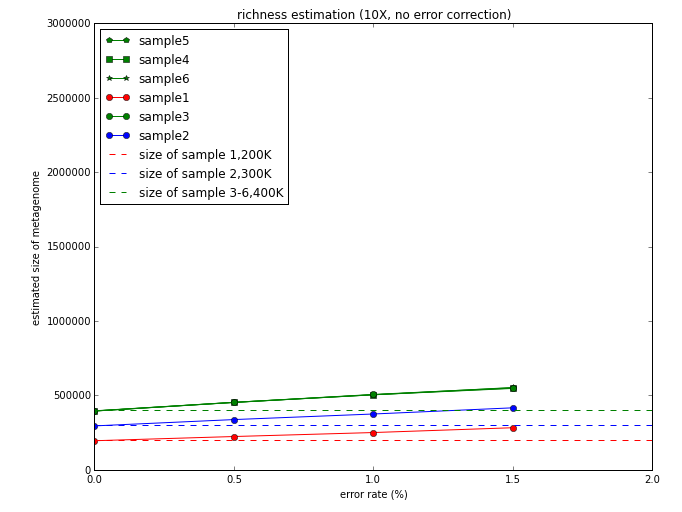
\includegraphics[width=4in]{./figures/IGS_richness_adjustment.png}}
\caption{\bf Richness estimation using IGS method adjusted by sequencing error
rate and false positive rate of bloom filter}
\label{fig:IGS_richness_adjustment}
\end{figure}

\subsubsection{comparison of dissimilarity matrix from beta diversity analysis}

To evaluate the effectiveness of beta diversity analysis using IGS based method, we compare the dissimilarity matrix generated by IGS based method with that generated from another metagenomics comparison tool - Commet(Compareads), and the true matrix,since we know exactly the species composition of the simulated data sets.

The clustering and ordination are all from the dissimilarity matrix. We think comparing matrix directly makes more sense than comparing the clustering and ordination plot. So we will not show the clustering and ordination figure in this evaluation. If the matrix can reflect the real relationship between samples reliably, the clustering and ordination will only be routine job.

The true dissimilarity matrix of the 6 simulated samples using bray-cutis metric from species composition directly is shown in Figure \ref{fig:simulated_real_matrix}.
For a simulated data set with 10x coverage and no error introduced (which will tell us the optimal performance of IGS method), the dissimilarity matrix can be calculated by using IGS method, as shown in Figure \ref{fig:simulated_matrix1}. We can see the absolute values in the matrix are not very close to that in the real matrix.But the relative values correspond to that in the real matrix well to show the relative distance between each pair of samples. To get a objective metric, we use 
Mantel (citing)test to calculate the correlation value between the two matrixes. The correlation is 0.9714, which means a very positive correlation between the two matrices. We are very confident that the matrix from IGS method can reflect the true relationship between samples pretty well.

Next we test how well the matrix calculated by various methods can reflect the real relationship between samples. 
The simulated data sets with sequencing depth as 1 and 10, with sequencing error as 3\% and without sequencing error are used in this experiment.
For the data sets with sequencing error, we use a HMM based error correction tool to preprocess the reads to check the effectiveness 
of error correction. We also  compare the performance of IGS based method and another metagenome comparing tool - Comet. 

As shown in Figure \ref{fig:IGS_correlation_methods}, firstly, for all data sets, the matrix from IGS method has a higher 
correlation to golden standard than that from Comet.  As expected, the matrix from data sets with sequencing error has a lower correlation than that from error-free
data sets. Also Comet is more sensitive to sequencing error rate, compared to IGS method.
However, error correction can increase the correlation significantly. Also higher coverage will yield more accurate matrix, which is not surprising.

Figure \ref{fig:IGS_correlation_coverage} shows how well the matrix calculated from data set with variable coverage can 
reflect the real relationship between samples. It is as expected that higher coverage data will yield better/more accurate distance matrix.
Note even with a coverage as low as 0.1, the correlation is 0.89. This can  give us the hint how reliable the result will be if 
we only use a small proportion of data from a large metagenomic data set.

% what if lower?? 0.01 for soil ?? 
% relationship between ordination/clustering and correlation??? 0.89, is it good enough to do ordination/clustering?


\begin{figure}[!ht]
 \centerline{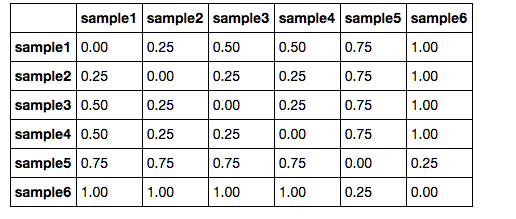
\includegraphics[width=4in]{./figures/simulated_real_matrix.png}}
\caption{\bf Dissimilarity matrix between synthetic samples using Bray-cutis from species composition directly }
\label{fig:simulated_real_matrix}
\end{figure}


\begin{figure}[!ht]
 \centerline{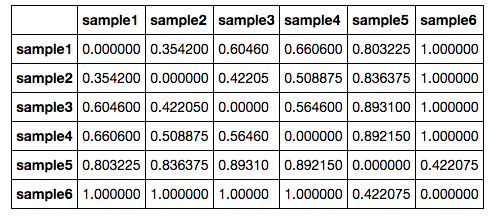
\includegraphics[width=4in]{./figures/simulated_matrix1.png}}
\caption{\bf Dissimilarity matrix between synthetic samples using Bray-cutis from sequencing reads using IGS method }
\label{fig:simulated_matrix1}
\end{figure}

\begin{figure}[!ht]
 \centerline{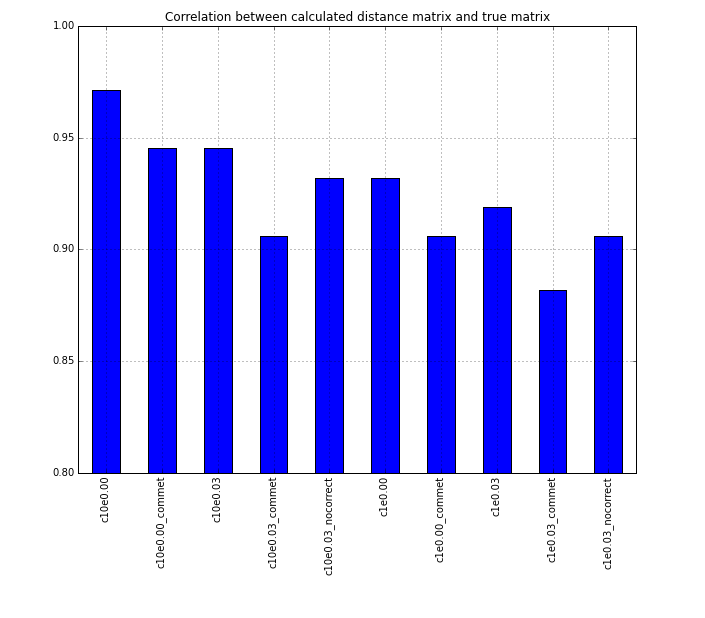
\includegraphics[width=4in]{./figures/IGS_correlation_methods.png}}
\caption{\bf Correlation between calculated distance matrix and true matrix from different data sets and using different methods}
\label{fig:IGS_correlation_methods}
\end{figure}


\begin{figure}[!ht]
 \centerline{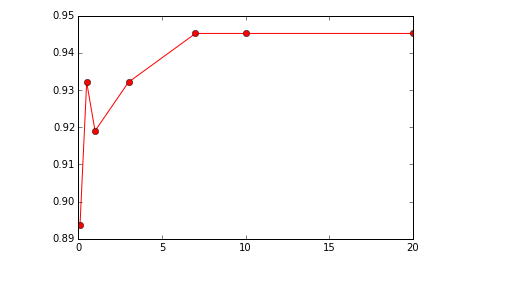
\includegraphics[width=4in]{./figures/IGS_correlation_coverage.png}}
\caption{\bf Correlation between calculated distance matrix and true matrix from different dat sets with different sequencing depth}
\label{fig:IGS_correlation_coverage}
\end{figure}


\subsubsection{Evaluate alpha diversity analysis by estimating size of metagenome}

We can use statistic metric to estimate the total number of IGSs in a sample, which can be used to calculate the estimated genome size of a sample using the formula below:
\\
size of genome = number of IGS x (reads\_length - k-size +1)\\
\\
Here we check how accurate the estimated size of genome and coverage is using different data sets with variable coverage/sequencing depth.

The genome size of the 6 samples should be:

sample1: AAAB 2x100K = 200K bp

sample2: AABC 3x100K = 300K bp

sample3: ABCD 4x100K = 400K bp

sample4: ABCE 4x100K = 400K bp

sample5: AFGH 4x100K = 400K bp

sample6: IFGH 4x100K = 400K bp

In this experiment, we use ACE metric since we find it is more accurate than Chao1, since it uses more abundance information.

Table \ref{fig:IGS_table_alpha1_10x_0} shows the estimated genome size of samples using error-free simulated sequencing data sets
is close to true size shown above. If the sequencing error is introduced, the estimated genome size is inflated dramatically as shown in Table \ref{fig:IGS_table_alpha1_10x_3_ne}, which is 
not surprising. However after applying error correction, we can still get good estimation of genome size, as shown in Table \ref{fig:IGS_table_alpha1_10x_3_e}.
This proves again error correction can improve the effectiveness of IGS method.

% test error rate 0.1?0.2?0.3? to see the influence of error rate???

Figure \ref{fig:IGS_table_alpha1_10x_3_e} shows the estimated genome size from data sets with variable coverage.
The estimated genome size keeps increasing as we use more reads, with higher coverage,which is  higher than actual genome size.
It's interesting that the estimated genome size is very high with low coverage, (probably due to more unique k-mers, which makes error correction more difficult. Then the estimated genome size drops a little bit as coverage from 0.1X to 1-3X, then starts to climb again as coverage increases, probably because there are always more erroneous k-mers that cannot be corrected. The good thing is that the climbing rate is not that high, this is believed to be due to the effectiveness of our error correction algorithms.

It is important to point that even though the absolute value of estimated genome size may be overestimated. The relative relationship between samples are reliable, as shown in the figure. Sample3,4,5,6 all have 4 species, while sample 2 has 3 species, and sample 1 has 2 species. They can be separately pretty well.


\begin{figure}[!ht]
 \centerline{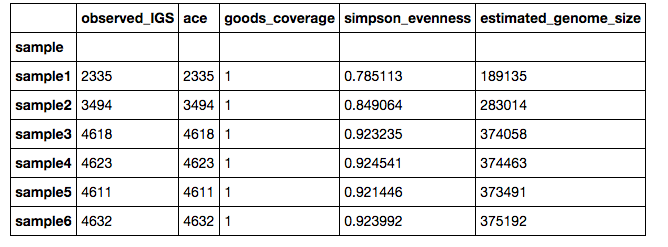
\includegraphics[width=4in]{./figures/IGS_table_alpha1_10x_0.png}}
\caption{\bf Coverage = 10x, No error}
\label{fig:IGS_table_alpha1_10x_0}
\end{figure}


\begin{figure}[!ht]
 \centerline{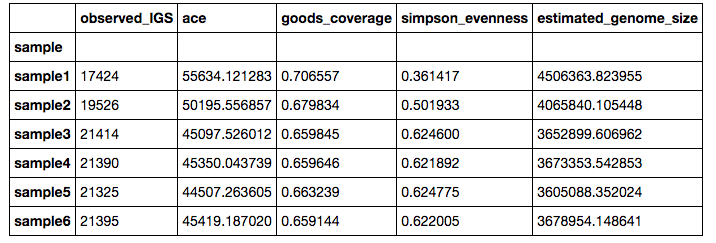
\includegraphics[width=4in]{./figures/IGS_table_alpha1_10x_3_ne.png}}
\caption{\bf Coverage = 10x, error = 3\%, no error correction}
\label{fig:IGS_table_alpha1_10x_3_ne}
\end{figure}



\begin{figure}[!ht]
 \centerline{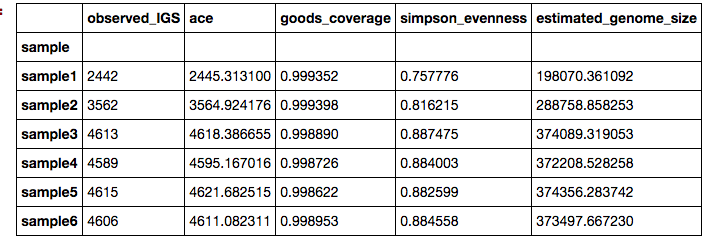
\includegraphics[width=4in]{./figures/IGS_table_alpha1_10x_3_e.png}}
\caption{\bf Coverage = 10x, error = 3\%, with error correction}
\label{fig:IGS_table_alpha1_10x_3_e}
\end{figure}

\begin{figure}[!ht]
 \centerline{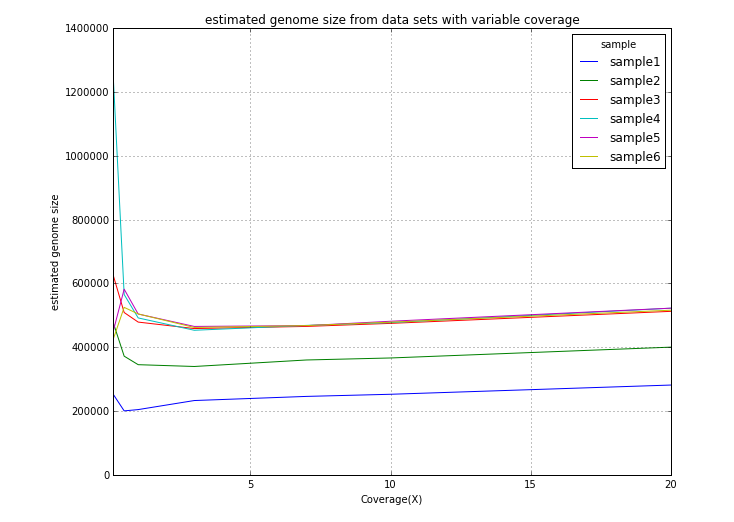
\includegraphics[width=4in]{./figures/IGS_figure_test_alpha.png}}
\caption{\bf estimated genome size from data sets with variable coverage}
\label{fig:IGS_figure_test_alpha}
\end{figure}


\subsection{The IGS method can provide a whole framework to do alpha or beta diversity, with good versatility.}

From the testing using simulated data sets shown here, we are confident that our IGS method works well and can give reliable results from data sets with error and low sequencing depth.

The IGS method can provide a whole framework to do alpha or beta diversity. Here we tested beta diversity using only bray-curtis metric and alpha diversity on richness only. Actually any metric can be applied to the IGS-by-samples table, abundance-based or incidence-baserd, richness or evenness.

Compareads(Commet) based on reads overlap between samples can get a matrix reflecting the real relationship between samples pretty good but it is stuck with one metric, which is based on the percentage of overlap reads between samples. This metric is like bray curtis , but not exactly the same.

\chapter{real data sets}

\section{Applying IGS method to real metagenome data sets}

Having shown that the IGS method gives good results about microbial diversity to simulated synthetic data sets, 
we will now evaluate the novel method on several published metagenomic datasets, with samples 
from ocean, human microbiome and soil. For the ocean sample and human microbiome data sets, we will compare the result from IGS method
with that from original publication. For soil sample, since there is no other diversity analysis that has been done
to these data sets, we will show the result we got from IGS and try to interpret the ecological meaning of the result.


\subsection{GOS data sets: Sorcerer II Global Ocean Sampling Expedition}

We tested the IGS method on a famous public dataset from the Sorcerer II Global Ocean Sampling expedition.
During the expedition, 44 water samples were collected from different locations across
Atlantic Ocean and Pacific Ocean and were sequenced using Sanger technology. The whole dataset is composed of XXXX reads, out of 44 samples.
A whole metagenomic comparison of the samples has been done
using a sequence alignment method in original research. 

The IGS method took XX hours on a XXX hardware to generate the dissimilarity matrix of the samples. After clustering, 
Figure \ref{fig:GOS-beta} shows that, consistently with the original study, the samples are clustered according to their 
geographical origin. The group with yellow color contains samples from Tropical- Galapogas. The group with light purple color
contains samples from Tropical -Open Ocean. The group with dark purple color contains samples from Sargasso. The group 
with green color contains samples from Temperate. 

If we compare the cluster we got from IGS method with the cluster in original study, we can see the IGS method yield a
cluster with better resolution and accuracy than the method used in original study. For example, in original study,
sample 14,21 and 22 from Tropical - Galapogas are separated from other Tropical- Galapagos samples, while in Figure \ref{fig:GOS-beta} 
they are grouped together. Also, samples 00a,00b,00c,00d, obviously from the same location, are grouped together in our result,while
in original research, sample 00a is separated from the other three samples.

Compared with the cluster by Compareads, our method is comparable, with some distinct differences. For example, sample 16 is clustered together with 15,17,18,19 in our result, but in the result by Compareads, sample 16 is clustered with 23,26 inaccurately, considering the geographical origin.

Next we use IGS method to analyze the alpha diversity. Figure \ref{fig:GOS-rarefaction} shows the rarefaction curve of IGSs of the samples.
As expected, we can not see the saturation,which means the sequencing data set is still far from enough overage. 
Because the data sets for different samples have dramatically different size, we estimate the total number of IGSs using Chao1 estimator with limited 
number of reads in each sample(50000) to make sure the smallest data set has enough reads for comparison, as shown in Figure \ref{fig:GOS-chao1} .

It is obvious that the richness of samples is related to the geographical origin. The sample from tropical area has a higher richness than
the samples from northern area. The relationship between samples is consistent to the cluster in beta diversity analysis shown above.

As discussed in the section above about alpha diversity analysis to synthetic data, such number of total IGSs may over-estimated but
the relative relationship between samples on richness should be reliable.

(This is not discussed in original research of GOS)

\begin{figure}[!ht]
 \centerline{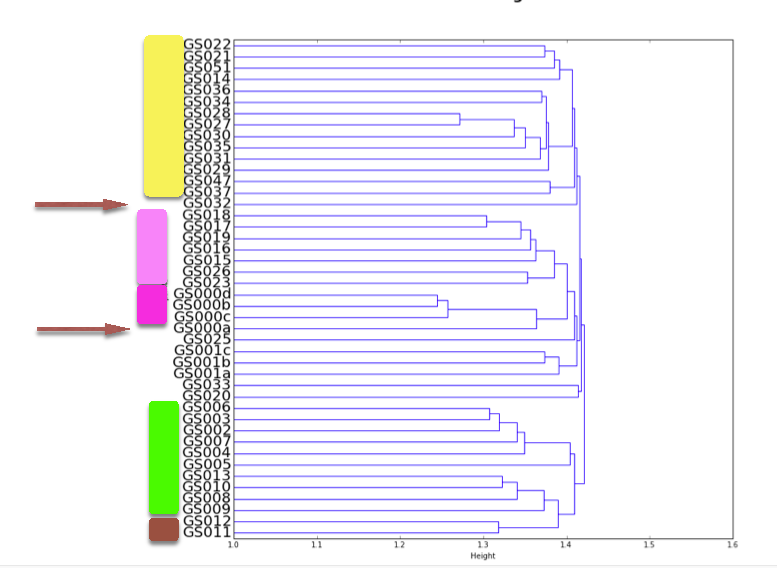
\includegraphics[width=7in]{./figures/GOS_cluster.png}}
\caption{\bf cluster of GOS samples using IGS method}
\label{fig:GOS-beta}
\end{figure}

\begin{figure}[!ht]
 \centerline{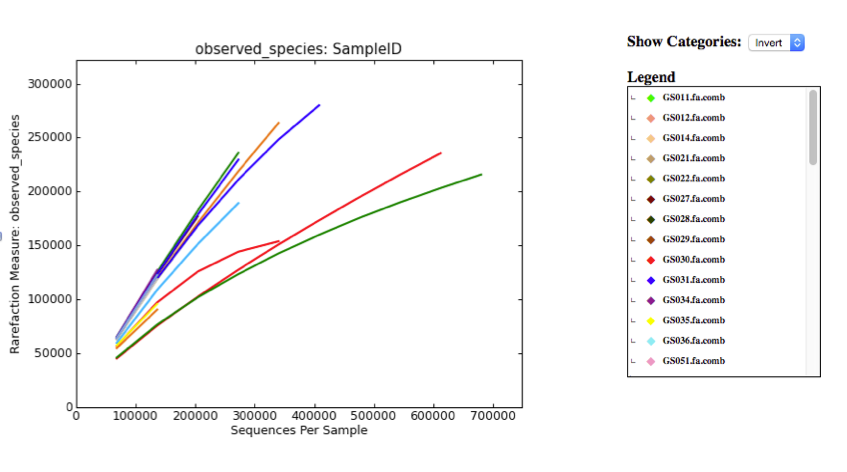
\includegraphics[width=7in]{./figures/GOS_observed.png}}
\caption{\bf Rarefaction curve of IGSs of the GOS samples}
\label{fig:GOS-rarefaction}
\end{figure}

\begin{figure}[!ht]
 \centerline{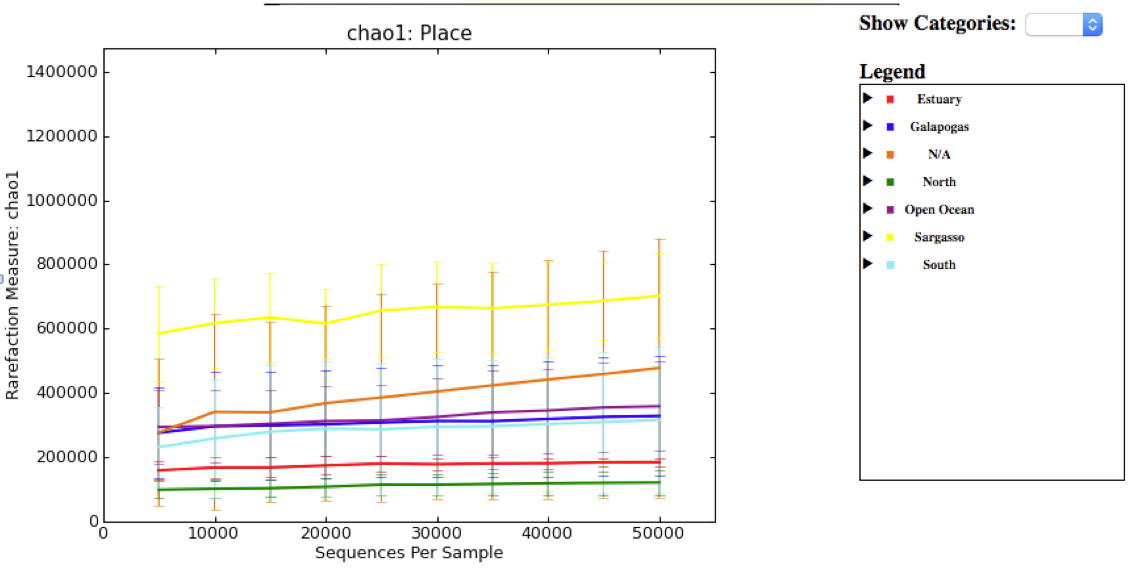
\includegraphics[width=7in]{./figures/GOS_chao.png}}
\caption{\bf Estimated number of IGSs of the GOS samples}
\label{fig:GOS-chao1}
\end{figure}


% result not good, remove it?
%\subsection{MetHit Human Gut metagenomics data set}


\subsection{HMP metagenomics data set}
% now have alpha and beta, smallest samples
% full sample 110 .... good for binning?
Here we test IGS method on 12 HMP(Human Microbiome Project) samples from different body parts like skin, oral or vaginal. 
Principal component analysis(Figure \ref{fig:HMP_beta}) shows the samples are separated well by the body parts where they are collected. (P value: XX)

Rarefaction curve and estimated number of IGSs shows the richness of samples is related to the body part where they are collected. The 
oral samples have higher richness than skin or vaginal samples, which is consistent  to other research. 



\begin{figure}[!ht]
 \centerline{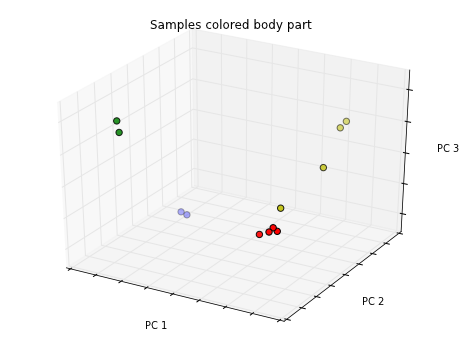
\includegraphics[width=7in]{./figures/HMP_beta.png}}
\caption{\bf PCoA of HMP}
\label{fig:HMP_beta}
\end{figure}

\begin{figure}[!ht]
 \centerline{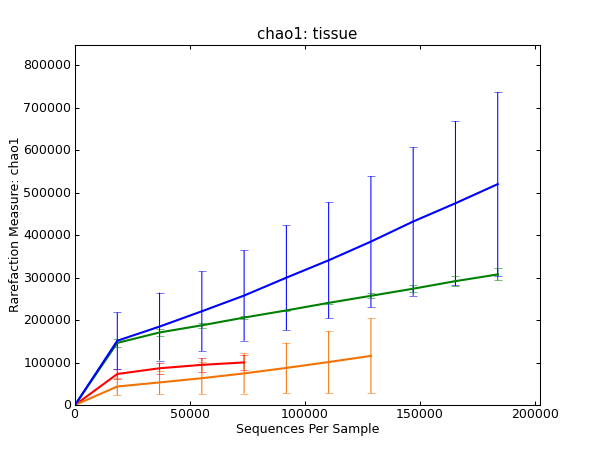
\includegraphics[width=7in]{./figures/HMP_alpha.png}}
\caption{\bf alpha diversity of HMP}
\label{fig:HMP_alpha}
\end{figure}





% ARMO subset 1m, Gpgc only 1m/2m subset, scalable??
\subsection{GPGC - Great Prairie Soil Metagenome Grand Challenge}

Having tested the IGS method on two relatively smaller metagenomic data sets, we will now use it to analyze 
a larger data set from soil samples collected from different treatment and different location across the great prairie region in the US. 
(Table \ref{table:gpgc}). 


%new GPGC has better understanding??

% should be enough??

Using 1m and 2m randomly selected subsets can yield pretty good results.

As discussed above with simulated data sets, using reads data sets with lower sequencing coverage will reduce
the accuracy of the analysis. But as shown in Figure \ref{fig:IGS_correlation_coverage}, with sequencing depth
as 0.1x, the calculated distance matrix using IGS method still has a reasonably high correlation with golden standard
distance matrix. So we can use subset of a large data set to acquire the diversity information, with the trade-off of
lower accuracy. 

For the GPGC datasets, we make a subset with 2 million reads from each sample and do the diversity analysis
using IGS method. 

Principal component analysis(Figure \ref{fig:GPGC_beta}) shows the samples are separated well by location where they are collected. (P value: XX)
This proves that the geographical origin plays a more important part in determining the similarity of genomic composition of samples, compared to different treatment. Note this is from a relatively small subset. (1-2 million reads). 

Figure \ref{fig:GPGC-alpha} shows the rarefaction curve and estimated number of IGSs of the samples. Basically the "corn" and "switchgrass' samples
have higher richness than "restored" and "prairie" samples. This observation that cultivation increases the richness of soil 
is consistent with the ?intermediate disturbance hypothesis?. The disturbance from treatment like cultivation opens more niches and the stable 
community like prairie eliminates some populations by the principle of competitive exclusion. . 

quotes TJ's comments - Its harder to explain the rank by state.  The Kansas site experiences more drought stress and higher temps. Maybe that selects for some more divergent physiologies? The Iowa and Wisconsin sites experience more cold, esp freezing conditions arresting their biology for 3-4 months, but the freeze-thaw cycles also kill off some each cycle (sound like intermediate disturbance!!), and with new growth each spring, this new growth would the fast growers, i.e. less diverse. Why Iowa is the least diverse, I don?t know - they planned it to help Adina and Titus with assembly.

 Also from the alpha diversity, we can have a rough estimation of the  total size of metagenome in iowa soil, which is about 540G basepairs. This 
 proves the high complexity of soil sample and we still need more sequencing effort to achieve a reasonable high coverage.
 

\begin{figure}[!ht]
 \centerline{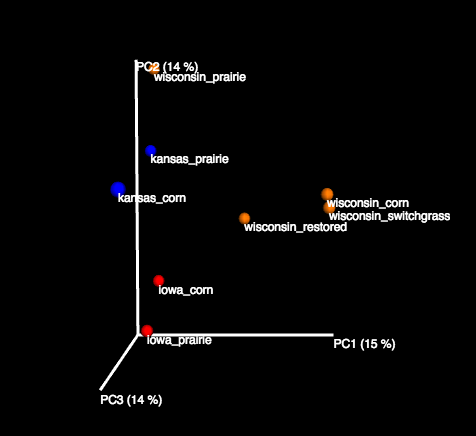
\includegraphics[width=4in]{./figures/GPGC_old_subset1M.png}}
\caption{\bf PCoA  of GPGC samples}
\label{fig:GPGC_beta}
\end{figure}



\begin{figure}[!ht]
 \centerline{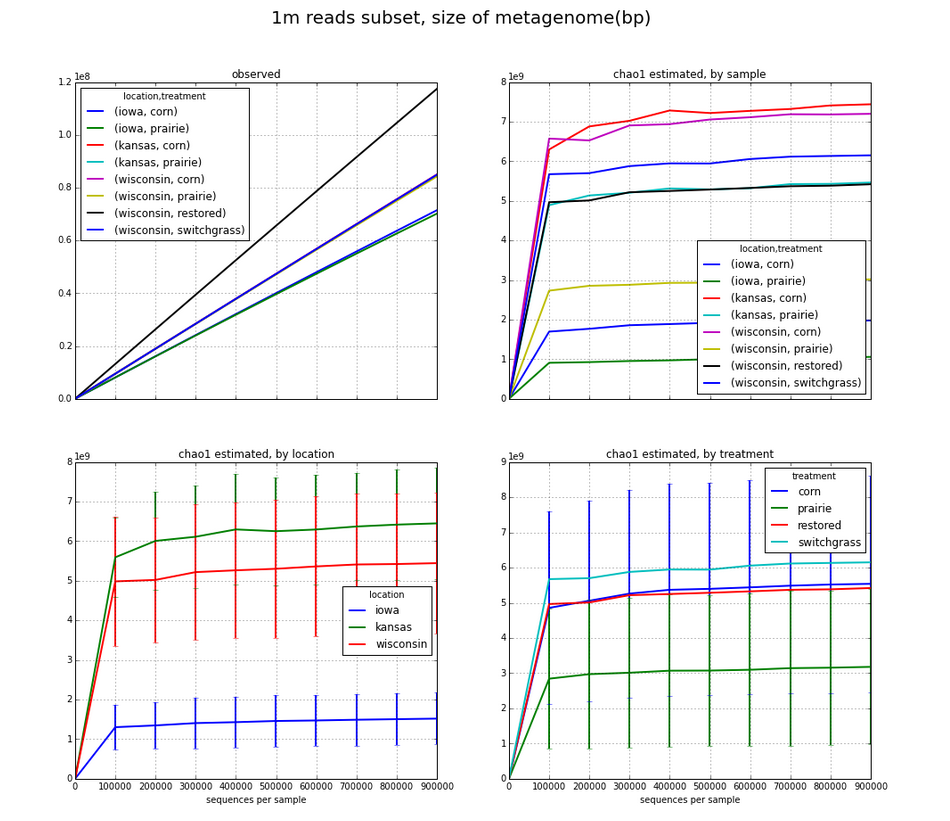
\includegraphics[width=7in]{./figures/GPGC_1m_old.png}}
\caption{\bf alpha diversity of GPGC samples}
\label{fig:GPGC-alpha}
\end{figure}



%\section{iterated diversity analysis}

%As we load more reads, we will see the separation more clearly. 

%simulated data sets. 

\subsection{more soil metagenomic samples}

Additionally we test the IGS method on two other unpublished data sets. One is a series of soil samples
collected from KBS with different treatment. Figure \ref{fig:KBS_beta} shows the IGS method can separate
the samples by treatment well. 

The other data set is a series of soil samples from Amazon rainforest. The samples are separated well
by the treatment. (Figure \ref{fig:ARMO_beta} ) It is also obvious that samples from forest have 
lower richness than prairie.  (Figure \ref{fig:ARMO_alpha})




\begin{figure}[!ht]
 \centerline{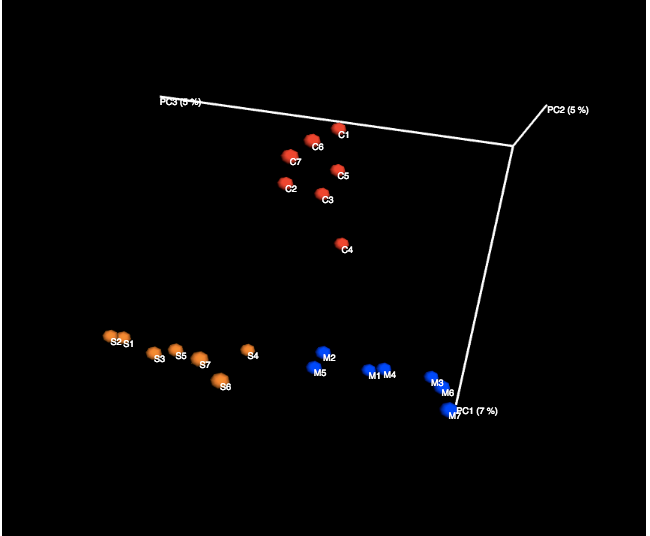
\includegraphics[width=4in]{./figures/IGS_KBS_beta.png}}
\caption{\bf PCoA of soil samples collected from KBS}
\label{fig:KBS_beta}
\end{figure}

\begin{figure}[!ht]
 \centerline{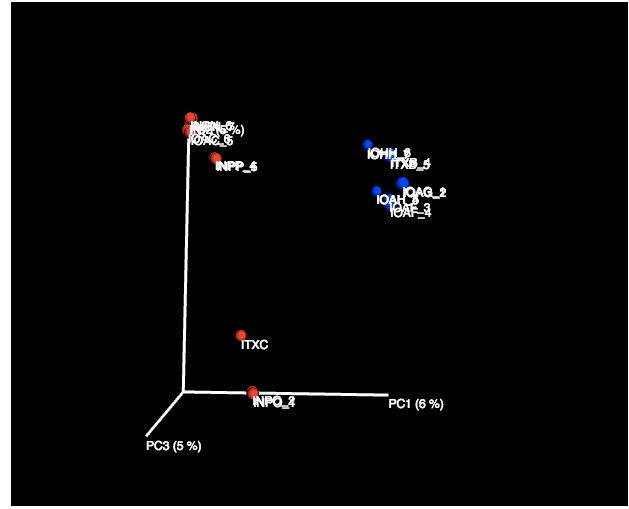
\includegraphics[width=4in]{./figures/IGS_ARMO_beta.png}}
\caption{\bf PCoA of soil samples collected from Amazon rainforest}
\label{fig:ARMO_beta}
\end{figure}

\begin{figure}[!ht]
 \centerline{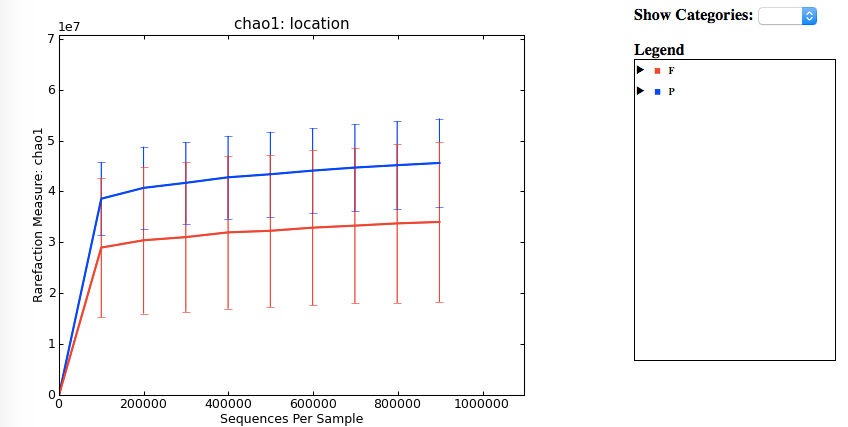
\includegraphics[width=7in]{./figures/IGS_ARMO_alpha.png}}
\caption{\bf PCoA of soil samples collected from Amazon rainforest}
\label{fig:ARMO_alpha}
\end{figure}

\section{Future Direction}

    - Extract reads that are unique/common between samples and do annotation to those reads.
    
    - sequencing depth evaluation
    
    - genome size estimation
    
    - better choosing diginorm parameters(size of hashtables, etc.) with genome size estimation as upper limit. 
    
    - reads binning/classification (after clustering)(if number of samples is small, may not be effective)
    
    - co assembly (by extracting the reads with total coverage across samples greater than 10, for example)
    
    - iterative diversity analysis - loading more reads to get higher accuracy, but  stops as pattern/clustering is significant enough
    (only for diversity analysis)
    
    
\section{Conclusion}

%Advantage:

%not only HMP, high depth, data
%but also low depth data, like soil metagenomics, which is impossible to use traditional method 



    

\section{Data}


\subsection{Four simulated reads data sets with different species abundance distribution}

\subsection{Simulated sequencing reads of e.coli}

Here we simulated 4 sequencing reads data sets with read length as 100bp of e.coli with different sequencing depth(50x and 150x) and different sequencing error rate(1\%,2\% and 0\%). Table \ref{table:ecoli}

\begin{table}[h]
\caption{
\bf{Simulated sequencing reads data sets of e.coli}
}
\begin{tabular}{|l|l|l|ll}
\cline{1-3}
sample & coverage & error rate &  &  \\ \cline{1-3}
A      & 150      & 0.01       &  &  \\ \cline{1-3}
B      & 50       & 0.01       &  &  \\ \cline{1-3}
C      & 50       & 0.01       &  &  \\ \cline{1-3}
D      & 50       & 0.02       &  &  \\ \cline{1-3}
\end{tabular}
\label{table:ecoli}
\end{table}



\begin{table}[h]
\caption{GPGC Data sets}
\label{my-label}
\begin{tabular}{|l|l|l|l|l|}
\hline
sample & \# of reads & size of .gz file & \# of bps & ave. length \\ \hline
iowa corn & 1514290825 & 46G & 144202427079 & 95.2 \\ \hline
iowa prairie & 2597093273 & 74G & 226815059143 & 87.3 \\ \hline
kansas\_corn & 2029883371 & 66G & 206933829048 & 101.9 \\ \hline
kansas\_prairie & 0 & 145G & 0 & 0 \\ \hline
wisconsin\_corn & 1616440116 & 51G & 162257698471 & 100.4 \\ \hline
wisconsin\_prairie & 1653557590 & 53G & 166467901724 & 100.7 \\ \hline
wisconsin\_restored & 226830595 & 11G & 34241520930 & 151.0 \\ \hline
wisconsin\_switchgrass & 310966735 & 13G & 40259619921 & 129.5 \\ \hline
\end{tabular}
\label{table:gpgc}
\end{table}

\chapter{Conclusion}

\section{Summary}

\section{Future Work}


\bibliography{dis}
\end{document}

    
